\subsection{Proxy}
\subsubsection{Định nghĩa}
Proxy là một mẫu thiết kế hướng đối tượng (design pattern) trong lập trình, thuộc nhóm mẫu cấu trúc (structural pattern). Nó cho phép bạn cung cấp một đối tượng trung gian (proxy) để kiểm soát quyền truy cập vào đối tượng thực (real object). Proxy hành động như một lớp ủy quyền và cung cấp một giao diện tương tự như đối tượng thực, cho phép kiểm soát và thực hiện các hoạt động bổ sung trước hoặc sau khi gọi đến đối tượng thực.
\subsubsection{Cách sử dụng}
Chúng ta có thể sử dụng proxy khi:
\begin{itemize}
    \item Khi bạn có một đối tượng dịch vụ nặng gây lãng phí tài nguyên hệ thống do luôn hoạt động, mặc dù thỉnh thoảng bạn chỉ cần nó.
    \item Khi bạn muốn chỉ những khách hàng cụ thể mới có thể sử dụng đối tượng dịch vụ.
    \item Khi bạn muốn che giấu thông tin về đối tượng thực khỏi người dùng, đặc biệt là trong trường hợp quyền truy cập hoặc bảo mật.
    \item Khi bạn muốn tạo ra các đối tượng khác nhau với chức năng tương tự, nhưng có quyền truy cập hoặc hành vi khác nhau.
\end{itemize}
\subsubsection{Cấu trúc}
\begin{itemize}
    \item Về lí thuyết, mẫu Proxy này tạo ra một class Proxy để ngắn cách người dùng truy cập trực tiếp vào đối tượng mà không thông qua lớp trung gian.
    \item Ở lớp Proxy này, ta có chứa cả đối tượng mà người dùng muốn truy cập.
\end{itemize}
Các thành phần chính của mẫu Proxy như sau:
\begin{itemize}
    \item ServiceInterface là một định nghĩa giao diện cho cả Proxy và Service để Proxy có thể được sử dụng bất kì nơi nào mà Service được mong đợi.
    \item Service là một class định nghĩa ServiceInterface mà Proxy đại diện.
    \item Proxy là một class có chứa một tham chiếu cho phép Proxy truy cập vào Service. 
\end{itemize}
\begin{center}
    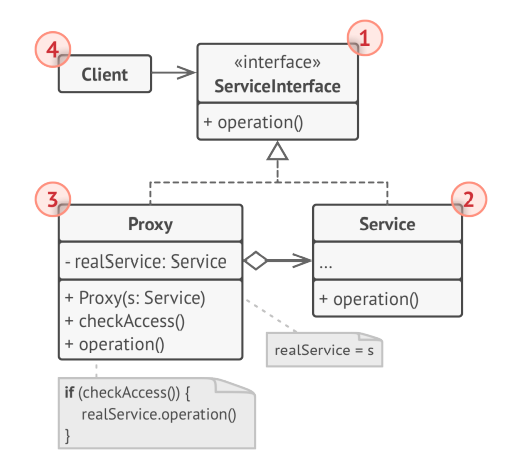
\includegraphics[scale=0.6]{image/structural/proxy.png}
\end{center}
\subsubsection{Ưu điểm và Nhược điểm}
Ta có các ưu nhược điểm sau:
Ưu điểm:
\begin{itemize}
    \item Proxy cho phép thêm các logic bổ sung mà không làm thay đổi đối tượng thực.
    \item Bảo vệ tính toàn vẹn của đối tượng thực bằng cách kiểm soát truy cập vào nó.
    \item Cung cấp một lớp trung gian để xử lý các yêu cầu phức tạp hoặc tốn nhiều tài nguyên của đối tượng thực.
\end{itemize}
Nhược điểm:
\begin{itemize}
    \item Tăng độ trễ trong việc gọi phương thức do cần thông qua lớp proxy.
\end{itemize}
\subsubsection{Code Example}
\begin{itemize}
    \item Ta có một ảnh thực, một ảnh proxy để kế thừa từ interface ảnh.
    \item Trong ảnh thực, ta có hàm trình bày và hàm tải từ đĩa.
    \item Ở cấu trúc trên, nếu chưa có ảnh nào được tải lên proxy thì lần truy cập đầu, proxy phải tải ảnh vào chỗ mình, các lần sau không cần thiết làm điều đó.
\end{itemize}
\begin{lstlisting}
#include <iostream>
#include <string>

// Common interface for the RealObject and Proxy
class Image {
public:
    virtual void display() = 0;
};

// RealObject
class RealImage : public Image {
private:
    std::string filename;

public:
    RealImage(const std::string& filename) : filename(filename) {
        loadFromDisk();
    }

    void display() override {
        std::cout << "Displaying image: " << filename << std::endl;
    }

    void loadFromDisk() {
        std::cout << "Loading image from disk: " << filename << std::endl;
    }
};

// Proxy
class ProxyImage : public Image {
private:
    std::string filename;
    RealImage* realImage;

public:
    ProxyImage(const std::string& filename) : filename(filename), realImage(nullptr) {}

    void display() override {
        if (realImage == nullptr) {
            realImage = new RealImage(filename);
        }
        realImage->display();
    }
};

int main() {
    // Use ProxyImage to create and display the image
    Image* image = new ProxyImage("image.jpg");

    // The first time displaying the image, it will load from disk
    image->display();

    // The second time displaying the image, it won't need to reload from disk
    image->display();

    delete image;

    return 0;
}


\end{lstlisting}
Ở hàm main, ta thực hiện tạo ảnh và display ảnh 2 lần. Ở lần đầu do phải tải ảnh lên proxy còn lần sau thì không cần thiết.\\
\newline
\textbf{Kết quả:}
\begin{lstlisting}
Loading image from disk: image.jpg
Displaying image: image.jpg
Displaying image: image.jpg
\end{lstlisting}
\subsubsection{Các Pattern liên quan}
\begin{itemize}
    \item Adapter để chuyển đổi các class còn Proxy tạo ra class để người dùng truy cập vào nó trước khi đụng được vào đối tượng thật. Chúng ta có thể kết hợp cả hai mẫu này như là để chuyển đổi giữa các Proxy.
    \item Decorator có cấu trúc giông với Proxy nhưng khác nhau về mục đích sử dụng. Decorator cho đối tượng thêm trách nhiệm còn Proxy thì kiểm soát quyền truy cập vào đối tượng.
\end{itemize}